\documentclass[aspectratio=169,10pt]{beamer}
\usepackage{theme/strawboss-theme}

\title{StrawBoss}
\author{}
\date{}

\begin{document}

% ================= 1. COPERTĂ =================
\begin{frame}[plain]
  \begin{tikzpicture}[remember picture,overlay]
    \fill[sbCream] (current page.south west) rectangle (current page.north east);
  \end{tikzpicture}
  \begin{textblock*}{2cm}(1.4cm,1.0cm)
    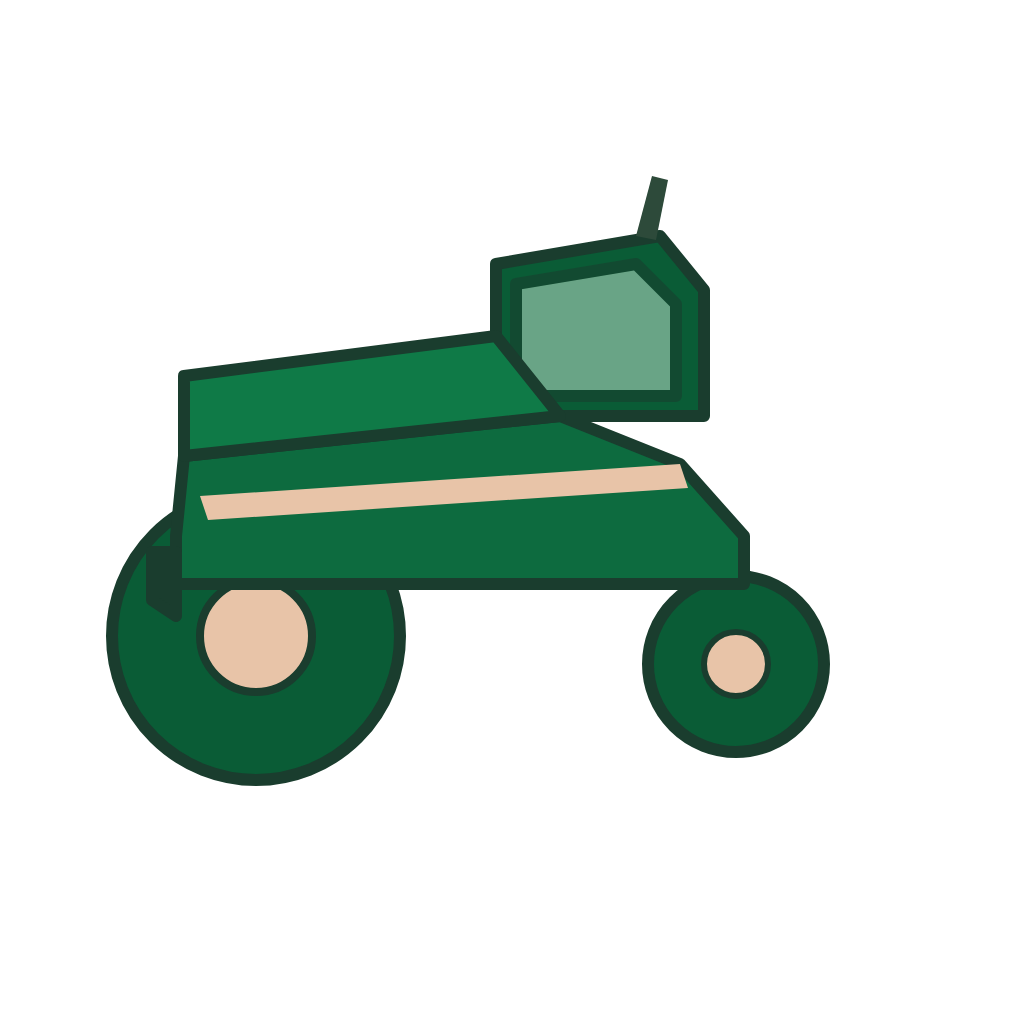
\includegraphics[width=1.3cm]{img/logo-tractor.png}
  \end{textblock*}
  \begin{textblock*}{6cm}(2.9cm,1.22cm)
    {\sffamily\Large\bfseries\color{sbInk} StrawBoss}
  \end{textblock*}

  \begin{textblock*}{13cm}(1.4cm,2.7cm)
    {\sbmonomed\small\color{sbTerra}\MakeUppercase{Logistica recoltei, de pe câmp până în depozit}}\par\vspace{0.35cm}
    {\rmfamily\fontsize{34}{40}\selectfont\color{sbInk} Vezi \textit{fiecare balot}, \textit{fiecare cursă}, \textit{fiecare leu.}}
  \end{textblock*}

  \begin{textblock*}{13cm}(1.4cm,7.3cm)
    \bigstat{291}{baloți urmăriți azi}
    \bigstat{65}{utilaje active}
    \bigstat{100\%}{traseu din GPS real}
  \end{textblock*}
\end{frame}

% ================= 2. PROBLEMA =================
\begin{frame}{Recolta se pierde acolo unde nu te uiți}
  \sbkicker{Problema}
  \begin{columns}[T]
    \begin{column}{0.55\linewidth}
      \vspace{0.4cm}
      \begin{itemize}
        \item Între câmp și depozit se pierd \textbf{4--12\% din baloți} — nimeni nu știe exact unde.
        \item Hârtii pierdute: avize, CMR-uri, bonuri de cântar — semnate pe hârtie, rătăcite în torpedou.
        \item Camioane care așteaptă degeaba pe câmp, în timp ce alte parcele stau nelucrate.
        \item Telefoane non-stop între birou și șoferi, doar ca să afli „unde ești acum?''
        \item La sfârșit de sezon, nimeni nu poate spune cu certitudine cât s-a produs, cât s-a livrat și cât s-a pierdut.
      \end{itemize}
    \end{column}
    \begin{column}{0.42\linewidth}
      \vspace{0.6cm}
      {\rmfamily\fontsize{22}{26}\selectfont\color{sbInk}\textit{„Câți baloți am făcut\\ luna asta?''}}\\[0.8cm]
      {\rmfamily\fontsize{22}{26}\selectfont\color{sbInk}\textit{Nimeni nu știe\\ sigur.}}
    \end{column}
  \end{columns}
\end{frame}

% ================= 3. SOLUȚIA =================
\begin{frame}{O singură platformă, tot lanțul}
  \sbkicker{Soluția}
  \vspace{0.2cm}
  \begin{center}
  {\sffamily\large\color{sbInk} Presare $\rightarrow$ Încărcare $\rightarrow$ Transport $\rightarrow$ Depozit $\rightarrow$ Rapoarte}
  \end{center}
  \vspace{0.5cm}
  \begin{columns}[T]
    \begin{column}{0.48\linewidth}
      {\sffamily\bfseries\color{sbTerra} Aplicația mobilă}\\[0.2cm]
      \begin{itemize}
        \item Pentru oamenii din teren: șoferi, operatori încărcare, presă, depozit.
        \item Funcționează \textbf{complet offline} — datele se sincronizează singure când revine semnalul.
        \item Butoane mari, ecran citibil în soare puternic.
      \end{itemize}
    \end{column}
    \begin{column}{0.48\linewidth}
      {\sffamily\bfseries\color{sbTerra} Dashboard-ul de birou}\\[0.2cm]
      \begin{itemize}
        \item Pentru dispecer și administrator: planificare, monitorizare \textbf{în timp real}, rapoarte, documente.
        \item Ecranul se actualizează singur — fără refresh, fără telefoane.
        \item Toate conturile în română și engleză.
      \end{itemize}
    \end{column}
  \end{columns}
\end{frame}

% ================= 4. CINE CE FOLOSEȘTE =================
\begin{frame}{Un ecran potrivit pentru fiecare rol}
  \sbkicker{Echipa}
  \vspace{0.3cm}
  \begin{columns}[T]
    \begin{column}{0.5\linewidth}
      {\sffamily\bfseries\small\color{sbMuted}\MakeUppercase{Mobil — teren}}\\[0.25cm]
      \begin{itemize}
        \item \textbf{Șofer} — transportă baloții de la câmp la depozit
        \item \textbf{Operator încărcare} — încarcă camioanele, numără baloții
        \item \textbf{Operator presă} — presează și înregistrează producția
        \item \textbf{Operator depozit} — confirmă livrările, cântărește
        \item \textbf{Planificator câmp} — desenează parcele și depozite
      \end{itemize}
    \end{column}
    \begin{column}{0.5\linewidth}
      {\sffamily\bfseries\small\color{sbMuted}\MakeUppercase{Web — birou}}\\[0.25cm]
      \begin{itemize}
        \item \textbf{Dispecer} — planifică ziua, urmărește cursele
        \item \textbf{Administrator} — tot ce face dispecerul, plus conturi, mașini, setări, rapoarte
        \item \textbf{Super administrator} — gestionează organizațiile și flota de telefoane
      \end{itemize}
      \vspace{0.4cm}
      {\sffamily\footnotesize\color{sbMuted} Restul acestei prezentări arată dashboard-ul de administrator — cel mai complet ecran din platformă.}
    \end{column}
  \end{columns}
\end{frame}

% ================= PARTEA 1 DIVIDER =================
\sectiondivider{Partea 1}{Dashboard-ul\\de birou}{Tot ce se întâmplă pe câmp, într-un singur ecran care se actualizează singur.}

% ---- 5. Command center ----
\begin{frame}{Toată ziua, pe un singur ecran}
  \sbkicker{Centru de comandă}
  \begin{columns}[T]
    \begin{column}{0.34\linewidth}
      \vspace{0.3cm}
      \begin{itemize}
        \item Hartă live cu parcele, utilaje și depozite
        \item Fluxul de curse active, actualizat singur — fără refresh
        \item Un click pe orice cursă $\rightarrow$ fișa completă
      \end{itemize}
    \end{column}
    \begin{column}{0.66\linewidth}
      \shotframe[\linewidth]{img/admin/command-center.jpg}
    \end{column}
  \end{columns}
\end{frame}

% ---- 6. Tasks ----
\begin{frame}{Planifici ziua în câteva minute}
  \sbkicker{Sarcini}
  \begin{columns}[T]
    \begin{column}{0.32\linewidth}
      \vspace{0.3cm}
      \begin{itemize}
        \item Vezi dintr-o privire câte prese, încărcătoare și camioane sunt în lucru azi
        \item Tablou \textbf{Planificat / În lucru / Finalizat}, actualizat live
        \item Atribui utilaje la parcele prin \textbf{drag \& drop}
      \end{itemize}
    \end{column}
    \begin{column}{0.68\linewidth}
      \shotframe[\linewidth]{img/admin/tasks.png}
    \end{column}
  \end{columns}
\end{frame}

% ---- 7. Map ----
\begin{frame}{Fiecare parcelă, fiecare depozit, fiecare utilaj — pe hartă}
  \sbkicker{Hartă}
  \begin{columns}[T]
    \begin{column}{0.32\linewidth}
      \vspace{0.3cm}
      \begin{itemize}
        \item Desenezi parcele și depozite direct pe hartă satelit
        \item \textbf{Suprafața în hectare se calculează automat} cât desenezi
        \item Vezi ferme, utilaje și depozite grupate, cu un click pe fiecare
      \end{itemize}
    \end{column}
    \begin{column}{0.68\linewidth}
      \shotframe[\linewidth]{img/admin/map.jpg}
    \end{column}
  \end{columns}
\end{frame}

% ---- 8. Curse (own fleet + aux) ----
\begin{frame}{Fiecare cursă, sub control — inclusiv transportatorii externi}
  \sbkicker{Curse}
  \begin{columns}[T]
    \begin{column}{0.32\linewidth}
      \vspace{0.3cm}
      \begin{itemize}
        \item \textbf{Două registre separate}: flota proprie și transportatorii externi
        \item Solicitările venite prin portal se \textbf{confirmă cu un click} — cursa se creează automat
        \item Evidențiere automată când lipsesc baloți față de cât s-a încărcat
      \end{itemize}
    \end{column}
    \begin{column}{0.68\linewidth}
      \shotframe[\linewidth]{img/admin/trips.png}
    \end{column}
  \end{columns}
\end{frame}

% ---- 9. Trip detail ----
\begin{frame}{Povestea completă a unei curse}
  \sbkicker{Fișa cursei}
  \begin{columns}[T]
    \begin{column}{0.32\linewidth}
      \vspace{0.3cm}
      \begin{itemize}
        \item Cronologie completă: încărcare, transport, sosire, livrare
        \item \textbf{Cele trei semnături}: operator încărcare, șofer, depozit
        \item CMR generat automat, descărcabil direct din fișă
      \end{itemize}
    \end{column}
    \begin{column}{0.68\linewidth}
      \shotframe[\linewidth]{img/admin/trip-detail.png}
    \end{column}
  \end{columns}
\end{frame}

% ---- 10. Trasee GPS ----
\begin{frame}{Kilometri reali, nu declarați}
  \sbkicker{Trasee}
  \begin{columns}[T]
    \begin{column}{0.32\linewidth}
      \vspace{0.3cm}
      \begin{itemize}
        \item Traseul fiecărui utilaj, din GPS-ul telefonului — nu din ce declară cineva
        \item Alege intervalul: ultima oră, zi, săptămână, lună sau personalizat
        \item Suprapui mai multe trasee simultan, cu legendă
      \end{itemize}
    \end{column}
    \begin{column}{0.68\linewidth}
      \shotframe[\linewidth]{img/admin/tracks.jpg}
    \end{column}
  \end{columns}
\end{frame}

% ---- 11. Rapoarte 1 ----
\begin{frame}{Rapoarte care răspund la „cât am produs și cât am pierdut?''}
  \sbkicker{Rapoarte}
  \begin{columns}[T]
    \begin{column}{0.32\linewidth}
      \vspace{0.3cm}
      \begin{itemize}
        \item \textbf{5 indicatori}: produs, încărcat, livrat, stoc depozit, procent pierdere
        \item \textbf{10 tab-uri}: ferme, câmpuri, depozite, clasamente, costuri, operatori și mai multe
        \item Export CSV curat, cu diacritice, deschis direct în Excel
      \end{itemize}
    \end{column}
    \begin{column}{0.68\linewidth}
      \shotframe[\linewidth]{img/admin/reports-ferme.png}
    \end{column}
  \end{columns}
\end{frame}

% ---- 12. Rapoarte 2 (costuri / operatori) ----
\begin{frame}{Costuri și oameni, negru pe alb}
  \sbkicker{Rapoarte — Costuri}
  \begin{columns}[T]
    \begin{column}{0.32\linewidth}
      \vspace{0.3cm}
      \begin{itemize}
        \item Motorină vs. consumabile vs. total, per utilaj
        \item Baloți per operator, sesiuni, medie pe sesiune
        \item Km per camion și per operator, cu acces direct la traseul din ziua respectivă
      \end{itemize}
    \end{column}
    \begin{column}{0.68\linewidth}
      \shotframe[\linewidth]{img/admin/reports-operatori.png}
    \end{column}
  \end{columns}
\end{frame}

% ---- 13. Alerte ----
\begin{frame}{Sistemul te anunță singur când ceva nu se leagă}
  \sbkicker{Alerte}
  \begin{columns}[T]
    \begin{column}{0.32\linewidth}
      \vspace{0.3cm}
      \begin{itemize}
        \item Nepotrivire de baloți la finalizarea cursei — alertă de fraudă
        \item Camion inactiv deși mai sunt baloți pe câmp
        \item O alertă neconfirmată nu se repetă la fiecare verificare
      \end{itemize}
    \end{column}
    \begin{column}{0.68\linewidth}
      \shotframe[\linewidth]{img/admin/alerts.png}
    \end{column}
  \end{columns}
\end{frame}

% ---- 14. Fișa mașinii ----
\begin{frame}{Fișa completă a fiecărui utilaj}
  \sbkicker{Mașini}
  \begin{columns}[T]
    \begin{column}{0.32\linewidth}
      \vspace{0.3cm}
      \begin{itemize}
        \item Ultima poziție GPS, activitate pe 7 zile, curse recente
        \item Consum de combustibil cu poze la bonuri
        \item Jurnal de alerte dedicat fiecărui utilaj
      \end{itemize}
    \end{column}
    \begin{column}{0.68\linewidth}
      \shotframe[\linewidth]{img/admin/machine-detail.png}
    \end{column}
  \end{columns}
\end{frame}

% ---- 15. Ferme ----
\begin{frame}{Ferme și câmpuri, fără birocrație}
  \sbkicker{Ferme}
  \begin{columns}[T]
    \begin{column}{0.32\linewidth}
      \vspace{0.3cm}
      \begin{itemize}
        \item Nume, telefon, CUI, cod APIA, adresă — toate într-un loc
        \item \textbf{Import KML} — încarci fișierul, previzualizezi parcelele
        \item Atribuire în masă a parcelelor neasignate
      \end{itemize}
    \end{column}
    \begin{column}{0.68\linewidth}
      \shotframe[\linewidth]{img/admin/farms.png}
    \end{column}
  \end{columns}
\end{frame}

% ---- 16. Conturi ----
\begin{frame}{Un cont nou în 30 de secunde}
  \sbkicker{Conturi}
  \begin{columns}[T]
    \begin{column}{0.32\linewidth}
      \vspace{0.3cm}
      \begin{itemize}
        \item Utilizator și PIN generate automat la creare
        \item Bulină de prezență live pentru fiecare cont
        \item Dezactivezi un cont $\rightarrow$ acesta pierde accesul în mai puțin de un minut
      \end{itemize}
    \end{column}
    \begin{column}{0.68\linewidth}
      \shotframe[\linewidth]{img/admin/accounts.png}
    \end{column}
  \end{columns}
\end{frame}

% ---- 17. Mesaje ----
\begin{frame}{Nimic nu se pierde tăcut}
  \sbkicker{Mesaje}
  \begin{columns}[T]
    \begin{column}{0.32\linewidth}
      \vspace{0.3cm}
      \begin{itemize}
        \item Monitor centralizat pentru email și SMS trimise automat
        \item Status pentru fiecare mesaj: în așteptare, trimis, livrat, eșuat
        \item Buton de reîncercare pentru mesajele eșuate
      \end{itemize}
    \end{column}
    \begin{column}{0.68\linewidth}
      \shotframe[\linewidth]{img/admin/messages.png}
    \end{column}
  \end{columns}
\end{frame}

% ---- 18. Depozite ----
\begin{frame}{Fiecare depozit, cu inventarul lui la zi}
  \sbkicker{Depozite}
  \begin{columns}[T]
    \begin{column}{0.32\linewidth}
      \vspace{0.3cm}
      \begin{itemize}
        \item Stoc, persoană de contact, ultima activitate — pentru fiecare depozit
        \item Depozitul confirmă livrarea doar când camionul e efectiv acolo
        \item Stocul scade automat la fiecare livrare ieșită
      \end{itemize}
    \end{column}
    \begin{column}{0.68\linewidth}
      \shotframe[\linewidth]{img/admin/deposits.png}
    \end{column}
  \end{columns}
\end{frame}

% ================= PARTEA 2 DIVIDER =================
\sectiondivider{Partea 2}{Aplicația\\mobilă}{Construită pentru oameni care lucrează pe câmp, nu în birou.}

% ---- 19. Mobil general ----
\begin{frame}{Construită pentru câmp, nu pentru birou}
  \sbkicker{Aplicația mobilă}
  \begin{columns}[T]
    \begin{column}{0.62\linewidth}
      \vspace{0.3cm}
      \begin{itemize}
        \item \textbf{Funcționează complet offline} — sincronizare automată când revine semnalul
        \item Butoane mari, tastatură numerică pentru introducere rapidă
        \item \textbf{Mod contrast ridicat} pentru soare puternic
        \item Se conectează cu utilizator + PIN de 4 cifre — rămâne conectat între reporniri
        \item O înregistrare trimisă de două ori nu se dublează niciodată
      \end{itemize}
    \end{column}
    \begin{column}{0.38\linewidth}
      \mobileshot{mobil-sync.png}{Bara de sincronizare}
    \end{column}
  \end{columns}
\end{frame}

% ---- 20. Șofer ----
\begin{frame}{Șofer — livrarea în 3 pași}
  \sbkicker{Rol: Șofer}
  \begin{columns}[T]
    \begin{column}{0.62\linewidth}
      \vspace{0.3cm}
      \begin{itemize}
        \item Livrare în 3 pași: greutate, poză bon de cântar, semnătură
        \item \textbf{Confirmare automată} la sosirea în depozit — geofence-ul detectează singur
        \item Fluxul e reluabil: dacă telefonul moare la jumătate, revine exact de unde a rămas
        \item ,,Loadere din apropiere'' — vede în timp real ce încărcătoare sunt prin zonă
      \end{itemize}
    \end{column}
    \begin{column}{0.38\linewidth}
      \mobileshot{sofer-livrare.jpg}{Ecran livrare — 3 pași}
    \end{column}
  \end{columns}
\end{frame}

% ---- 21. Operator încărcare ----
\begin{frame}{Operator încărcare — zero selecție manuală}
  \sbkicker{Rol: Operator încărcare}
  \begin{columns}[T]
    \begin{column}{0.62\linewidth}
      \vspace{0.3cm}
      \begin{itemize}
        \item Câmpul activ se detectează automat prin GPS — niciodată ales manual
        \item Limită de baloți pe camion, configurabilă per mașină
        \item Scanează CMR-ul pe hârtie cu camera — se transformă automat în PDF
        \item ,,Mai vine un camion?'' — răspunde Da/Nu, sistemul cheamă șoferul automat
      \end{itemize}
    \end{column}
    \begin{column}{0.38\linewidth}
      \mobileshot{loader-camioane.png}{Camioane la loader}
    \end{column}
  \end{columns}
\end{frame}

% ---- 22. Operator presă ----
\begin{frame}{Operator presă — o singură tastatură mare}
  \sbkicker{Rol: Operator presă}
  \begin{columns}[T]
    \begin{column}{0.62\linewidth}
      \vspace{0.3cm}
      \begin{itemize}
        \item Tastatură numerică mare pentru numărul de baloți
        \item \textbf{Mod „Câmp activ''} — ecran minimal, rămâne aprins permanent
        \item Confirmare automată la intrarea pe câmp, alertă sonoră la ieșire
        \item Alege explicit \textbf{Parțial sau Total} — nimic presupus automat
      \end{itemize}
    \end{column}
    \begin{column}{0.38\linewidth}
      \mobileshot{presa-productie.png}{Mod câmp activ}
    \end{column}
  \end{columns}
\end{frame}

% ---- 23. Operator depozit ----
\begin{frame}{Operator depozit — confirmare doar la fața locului}
  \sbkicker{Rol: Operator depozit}
  \begin{columns}[T]
    \begin{column}{0.62\linewidth}
      \vspace{0.3cm}
      \begin{itemize}
        \item Vede totalul de baloți și tone din depozit, actualizat la fiecare livrare
        \item Confirmarea se deblochează \textbf{doar când camionul e efectiv la depozit}
        \item Greutate brută + tară, cu net calculat automat; comutator „cântar stricat'' pentru când echipamentul cade
        \item Funcționează complet offline, fără GPS suplimentar de la operator
      \end{itemize}
    \end{column}
    \begin{column}{0.38\linewidth}
      \mobileshot{depozit-confirmare.png}{Confirmare livrare}
    \end{column}
  \end{columns}
\end{frame}

% ---- 24. Planificator câmp ----
\begin{frame}{Planificator câmp — desenezi ca pe Google Earth}
  \sbkicker{Rol: Planificator câmp}
  \begin{columns}[T]
    \begin{column}{0.62\linewidth}
      \vspace{0.3cm}
      \begin{itemize}
        \item Desenezi parcele direct pe hartă satelit, punct cu punct
        \item Suprafața în hectare se calculează automat, live
        \item Terenul desenat apare imediat pe hartă, chiar și fără semnal
        \item Creezi ferme și atribui parcele direct din teren
      \end{itemize}
    \end{column}
    \begin{column}{0.38\linewidth}
      \mobileshot{geo-desen.jpg}{Desen parcelă}
    \end{column}
  \end{columns}
\end{frame}

% ================= 25. AUTOMATIZĂRI =================
\begin{frame}{Automatizări care lucrează în locul tău}
  \sbkicker{Sub capotă}
  \vspace{0.3cm}
  \begin{columns}[T]
    \begin{column}{0.5\linewidth}
      \begin{itemize}
        \item \textbf{Geofence automat} — detectează intrarea/ieșirea de pe parcelă sau din depozit, cu toleranță la eroarea GPS
        \item \textbf{CMR generat automat}, în două etape: la plecare și la sosire
        \item ,,Camion se apropie'' — încărcătorul e anunțat cu 5 km înainte
      \end{itemize}
    \end{column}
    \begin{column}{0.5\linewidth}
      \begin{itemize}
        \item Reconciliere orară: produs vs. încărcat vs. livrat, alertă la nepotriviri imposibile
        \item Camion inactiv — alertă către birou la 5 minute
        \item O cursă finalizată poate genera automat următoarea tură, pe același câmp
      \end{itemize}
    \end{column}
  \end{columns}
\end{frame}

% ================= 26. SYNC & SECURITATE =================
\begin{frame}{Nimic nu se pierde, nimic nu se dublează}
  \sbkicker{Fiabilitate}
  \vspace{0.3cm}
  \begin{columns}[T]
    \begin{column}{0.5\linewidth}
      \begin{itemize}
        \item Fiecare organizație e complet separată — propriile conturi, propriile date
        \item \textbf{Nimic nu se șterge definitiv} — totul rămâne recuperabil
        \item Jurnal de audit — cine, ce și când, imposibil de modificat
      \end{itemize}
    \end{column}
    \begin{column}{0.5\linewidth}
      \begin{itemize}
        \item Protecție împotriva ghicirii PIN-urilor pe portalurile publice
        \item Un cont dezactivat pierde accesul în mai puțin de un minut
        \item Aplicația și dashboard-ul sunt disponibile în română și engleză
      \end{itemize}
    \end{column}
  \end{columns}
\end{frame}

% ================= 27. FLOTĂ DE TELEFOANE =================
\begin{frame}{Telefoanele se administrează singure}
  \sbkicker{Management flotă}
  \vspace{0.3cm}
  \begin{itemize}
    \item Pentru parcuri de telefoane dedicate: aplicația \textbf{se actualizează singură}, fără magazin de aplicații
    \item Nu poate fi închisă forțat, dezinstalată sau dezactivată din greșeală de utilizator
    \item Permisiuni acordate automat la instalare, inclusiv locația în fundal
    \item Diagnostic la distanță — starea fiecărui telefon, vizibilă din birou
    \item Comenzi la distanță: repornire, colectare jurnale, reinstalare
  \end{itemize}
\end{frame}

% ================= 28. ÎNCHIDERE =================
{\setbeamertemplate{footline}{}
\begin{frame}[plain]
  \begin{tikzpicture}[remember picture,overlay]
    \fill[sbInk] (current page.south west) rectangle (current page.north east);
  \end{tikzpicture}
  \begin{textblock*}{2cm}(1.4cm,1.0cm)
    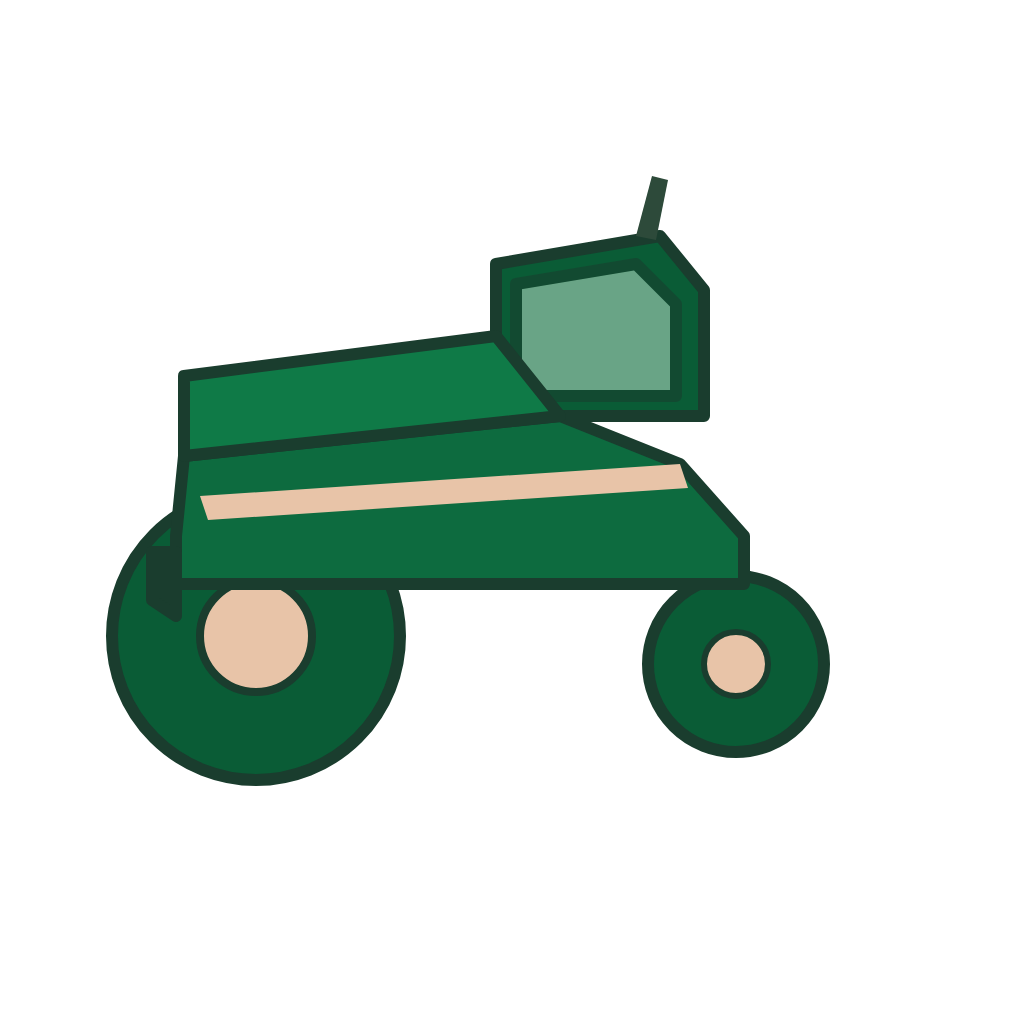
\includegraphics[width=1.3cm]{img/logo-tractor.png}
  \end{textblock*}
  \begin{textblock*}{11cm}(1.4cm,3.0cm)
    {\rmfamily\fontsize{34}{40}\selectfont\color{sbCream} Hai să vedem cum ar arăta\\ pe datele voastre.}
  \end{textblock*}
  \begin{textblock*}{11cm}(1.4cm,5.6cm)
    {\sffamily\color{sbGold}\large StrawBoss}\\[0.2em]
    {\sffamily\color{sbMuted} Logistica recoltei, de pe câmp până în depozit.}
  \end{textblock*}
\end{frame}}

\end{document}
